\selectlanguage{swedish}
\section{Polymerisering}
Den syntetiska processen att länka samman monomerer till polymera kedjor, kallas för polymerisation. Detta kan göras genom olika typer utav kem\-iska mekanismer, vilka kan delas in i fyra kategorier: Stegvis.., Kedjevis.., Ringöpnings.. och övriga polymerisationstekniker \cite[s. 117]{polym}.

Oavsett teknik så handlar polymerisation om att monomerer kopplas samman till polymerer. Detta sker genom att monomerer adderas till en växande polymerkedja. Detta kan ske på två sätt: antingen genom att en monomer adderas i taget, eller genom att flera monomerer adderas samtidigt. I det första fallet talar vi om stegvis polymerisation, och i det andra fallet talar vi generellt om kedjevis polymerisation.

Vårt huvudfokus kommer att ligga på stegvis polymerisation och kedjevis polymerisation, två helt olika processer som är mycket vanliga ute i industrin \cite[s. 131]{polym}. Notera att kedjevis polymerisation är ett samlingsnamn för tre principiellt liknande processer: radikal.., jon.. och koordinationspolymerisation. Trädet nedan visualiserar den beskrivna kategoriseringen av polymerisationstekniker.

\begin{figure}[ht]
    \centering
    % Träddiagram av polymeriserings typerna:
%Ref: PolyT p. 117
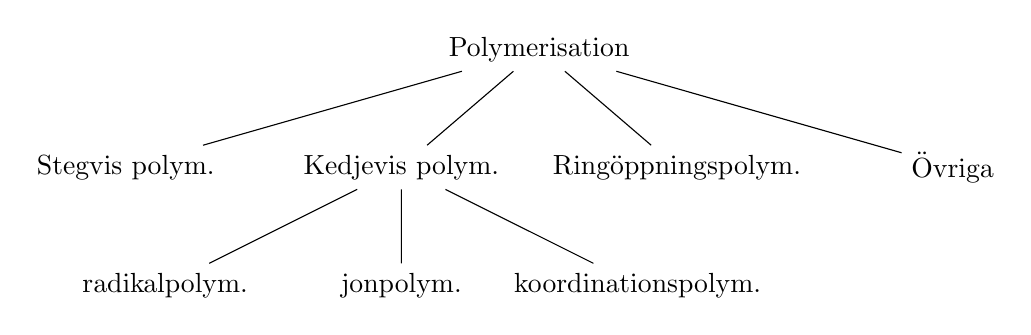
\begin{tikzpicture}[
    level 1/.style={sibling distance=3.5cm},
    level 2/.style={sibling distance=3cm},
    level 3/.style={sibling distance=3cm}
  ]
    \node {Polymerisation}
        child { node {Stegvis polym.}
        }
        child { node {Kedjevis polym.}
            child { node {radikalpolym.} }
            child { node {jonpolym.} }
            child { node {koordinationspolym.} }
        }
        child { node {Ringöppningspolym.}
        }
        child { node {Övriga}
        };
\end{tikzpicture}
    \caption{Kategorisering av polymerisationstekniker \cite[s.117]{polym}}
    \label{fig:polymerisations_typer}
\end{figure}

Polymeriseringsprocesser
\subsection{Stegvis polymerisation}
%Ethene chemfig



\subsection{Kedjevis polymerisation}
\subsubsection{Radikalpolymerisation}
\subsubsection{Jonpolymerisation}
\subsubsection{Koordinationspolymerisation}
\subsection{Ringöppningspolymerisation}
\subsection{Övriga polymerisationstekniker}